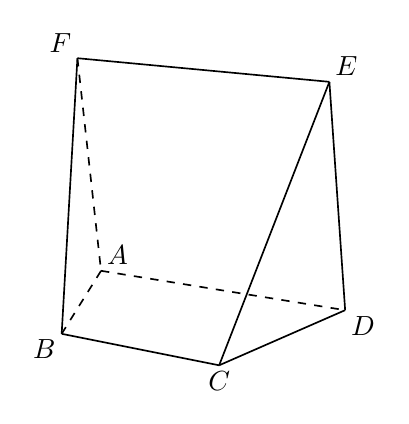
\begin{tikzpicture}[x=1cm,y=1cm,font=\normalsize,
  geometry edge/.style={solid,line width=.6pt},
  geometry label/.style={font=\normalsize,inner sep=2pt}]
\coordinate (B) at (0,0);
\coordinate (C) at (2,-0.4);
\coordinate (D) at (3.6,0.3);
\coordinate (E) at (3.4,3.2);
\coordinate (F) at (0.2,3.5);
\coordinate (A) at (0.5,0.8);
\draw[geometry edge] (F)--(E);
\draw[geometry edge] (E)--(D);
\draw[geometry edge] (E)--(C);
\draw[geometry edge] (D)--(C);
\draw[geometry edge] (C)--(B);
\draw[geometry edge] (B)--(F);
\draw[geometry edge,dashed] (F)--(A);
\draw[geometry edge,dashed] (A)--(B);
\draw[geometry edge,dashed] (A)--(D);
\node[geometry label,above left] at (F) {$F$};
\node[geometry label,above right] at (E) {$E$};
\node[geometry label,below right] at (D) {$D$};
\node[geometry label,below] at (C) {$C$};
\node[geometry label,below left] at (B) {$B$};
\node[geometry label,above right] at (A) {$A$};
\end{tikzpicture}
